3as\section{The \sys\ Framework Design and Implementation}
\label{sec:schedcp_framework}

\begin{figure}
    \centering
    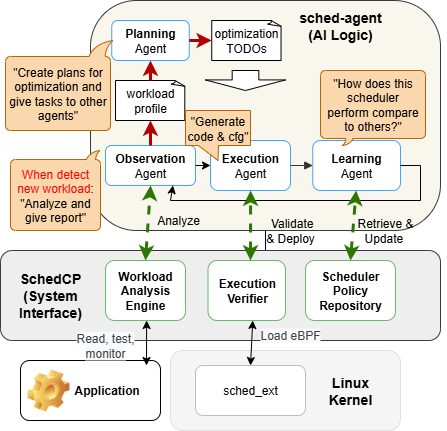
\includegraphics[width=0.9\columnwidth]{sections/img/arch-scheddcp.png}
    \caption{
        \textbf{The overall architecture, showing the separation of concerns between \sys\ and \agent.} 
        The \textbf{\sys} framework (bottom) acts as a safe system interface, providing tools to analyze workloads, verify code, and manage scheduler policies in the Linux kernel via eBPF.
        The \textbf{\agent} framework (top) contains the AI logic, where specialized agents for Observation, Planning, Execution, and Learning collaborate in a closed loop to autonomously create, deploy, and refine scheduling policies. The red line indicate the initialize process When \sys detects a new workload. The back arrow indicate the optimization loops, where \agent continue refines scheduler policies based on optimization plan and observation results.
    }
    \label{fig:frameworkarch}
\end{figure}

Our approach to agentic OS optimization is founded on a clean separation between the systems infrastructure and the AI logic, as illustrated in Figure~\ref{fig:frameworkarch}. We introduce \sys, a stable and secure control plane that acts as an 'API for OS optimization.' Our research is motivated by the insight that AI agents are fundamentally context engineering systems; like human experts, they need the right tools to gather information and act without being overwhelmed by prohibitive costs or irrelevant data. Therefore, as system researchers, our goal is not to build better AI agents, but to design superior systems and interfaces for them. \sys embodies this by providing the essential tools and safety guarantees for any agent to interact with the Linux kernel's scheduler, analogous to how a reinforcement learning framework provides an environment for an agent to learn. This section details \sys's design principles, core components, and implementation.

\subsection{Design Principles}
The design of \sys\ is governed by four key principles that ensure it is safe, efficient, and future-proof.

\textbf{Decoupling and Role Separation}: A system tightly coupled to a specific AI model's capabilities will quickly become obsolete as models evolve. To ensure our framework is future-proof, we believe the system's role must be separated from the AI's. Our principle is to decouple ``what to optimize'' (the AI's domain) from ``how to observe and act'' (the system's domain). We treat the AI agent as a performance engineer using a stable set of tools provided by the system, allowing the framework to remain relevant even as AI capabilities advance.

\textbf{Safety-First Interface Design}: Autonomous agents with kernel access pose inherent risks. System stability is non-negotiable, so we treat AI as potentially non-cautious actors and design defensive interfaces. The framework prevents catastrophic failures by default rather than trusting agents to avoid them.

\textbf{Context and Feedback Balance}: LLM agents face constraints from finite context windows and token costs. Performance degrades when flooded with irrelevant data. We address this through adaptive context provisioning: agents start with minimal summaries and progressively request details as needed, balancing cost against precision.

\textbf{Composable Tool Architecture}: Rigid workflows stifle LLMs' ability to reason and devise novel solutions. Following Unix philosophy, we provide atomic tools and let agents construct complex workflows through their reasoning capabilities, enabling novel solution generation.

\subsection{Core Components and Implementation}
\sys is engineered as a modular control plane, exposing its services to AI agents via the standard Model Context Protocol (MCP)~\cite{anthropic2024mcp}. This design cleanly separates the high-level policy orchestration managed by the agent from the low-level observation and execution handled by the framework, and avoids granting `root' privileges to the agent. The architecture consists of three primary services.

\textbf{1. Workload Analysis Engine.} This service provides agents with tiered access to system performance data. It offers three levels of information: (1) cost-effective API endpoints delivering pre-processed summaries like CPU load and memory usage, (2) secure sandbox access to basic file reading, application building, standard Linux profiling tools (\texttt{perf}, \texttt{strace}) and dynamically attachable eBPF probes for detailed analysis, and (3) a feedback channel that reports post-deployment performance metrics such as percentage change in makespan or latency. The service implements adaptive context provisioning, allowing agents to request progressively detailed information as needed.

\textbf{2. Scheduler Policy Repository.} This service is a vector database storing eBPF scheduler code with rich metadata: natural language descriptions, target workloads, and historical performance metrics. It provides APIs for semantic search and retrieval, enabling agents to find relevant schedulers or composable code primitives. To support system evolution, it includes endpoints for updating performance metrics and promoting new policies. The repository reduces generation costs by allowing reuse of proven solutions while maintaining a growing library of scheduling strategies.

\textbf{3. Execution Verifier.} This validation pipeline service accepts code artifacts and applies multi-stage verification. Stage one performs static analysis: eBPF verifier simulation and complexity analysis to catch safety violations and estimate overhead. Stage two conducts dynamic validation: compilation and execution within a micro-VM against correctness and performance tests. Upon passing both stages, the service issues a signed deployment token. The final stage provides canary deployment monitoring with a circuit breaker that automatically reverts to the last known-good scheduler if performance thresholds are breached. This implements our safety-first principle by ensuring all code undergoes rigorous vetting before production deployment.

\section{\agent: A Multi-Agent Framework for OS Optimization}
\label{sec:sched_agents}

Building on \sys, we developed \textbf{\agent}, a multi-agent AI framework for scheduler optimization. We implemented it using Claude Code's subagent architecture~\cite{anthropic2024subagents}, which provides specialized AI assistants with customized system prompts, tools, and separate context windows~\cite{anthropic2024multiagent}. This decomposes complex reasoning into manageable roles, mirroring expert human teams. Each agent handles one optimization stage: observation, planning, execution, and learning.

\subsection{Agent Roles and Responsibilities}

\subsubsection{Observation \& Analysis Agent - Building a Workload Profile}

The \textbf{Observation Agent} builds a comprehensive ``Workload Profile'' by strategically querying the Workload Analysis Engine. Its reasoning process determines the analysis sequence: starting with high-level summaries, then requesting deeper profiling based on initial findings. For example, after identifying a parallel build process through initial queries, the agent decides to request CPU statistics via \texttt{perf stat} and dependency traces via \texttt{strace}. The agent synthesizes these data points into a description of the workload in natural language, quantified performance characteristics, and explicit optimization goals. It manages the cost-precision tradeoff by requesting only essential information and can register for event notifications to trigger re-analysis when workload patterns change.

\subsubsection{Planning Agent - Policy Synthesis and Selection}

The \textbf{Planning Agent} transforms the Workload Profile into an optimization strategy. It constructs semantic queries for the Scheduler Policy Repository based on the profile's keywords and performance goals. The agent's decision logic follows a hierarchy: search for exact matches, broaden to similar patterns if needed, then decide among three pathways. For existing production-ready scheduler solutions with strong performance history, it configures parameters. For partial matches, it retrieves code and generates patches. When no suitable base exists, it composes new schedulers from algorithm primitives. The agent evaluates tradeoffs between reuse efficiency and customization needs using historical performance data from the repository.

\subsubsection{Execution Agent - Validated Policy Deployment}

The \textbf{Execution Agent} manages the development, validation and deployment process. It synthesizes code artifacts based on the Planning Agent's strategy, then submits them to the Execution Verifier. The agent interprets validation results and adapts accordingly: when static analysis fails, it refines the code; when dynamic tests fail, it analyzes errors and fixes logic issues. The agent decides whether to proceed, retry, or abandon approaches based on verifier feedback. Upon receiving a deployment token, it initiates canary rollout. If the circuit breaker triggers, the agent captures failure context and determines next steps, either revising the approach or escalating to the Learning Agent.

\subsubsection{Learning Agent - Performance Analysis and Knowledge Update}

The \textbf{Learning Agent} analyzes deployment outcomes to improve future performance. It retrieves metrics from the Feedback Channel and identifies success patterns and failure modes. For immediate benefit, it informs subsequent optimization cycles within the current session. For long-term improvement, it updates the Scheduler Policy Repository: refining performance metrics, annotating schedulers with deployment contexts, and promoting successful novel policies. The agent documents antipatterns from failures to prevent repetition. This dual approach enables both in-session adaptation and persistent system-wide learning.


\subsection{Example: Kernel Compilation}

To illustrate how these four agents work together, consider a kernel compilation workload. The \textbf{Observation Agent} begins by analyzing the Linux kernel source tree, executing \texttt{make -j} to understand the build process, and running \texttt{perf stat} to profile resource usage. This observation produces a Workload Profile: ``CPU-intensive parallel compilation task with short-lived processes, inter-process dependencies, and a goal to minimize makespan.'' During planning, the \textbf{Planning Agent} queries the Scheduler Policy Repository with keywords like ``throughput'' and ``compilation,'' retrieving \texttt{scx\_rusty} as a starting point. It generates a patch to make the scheduler dependency-aware. In execution, the \textbf{Execution Agent} submits the patched code to the Execution Verifier for validation, receiving a deployment token upon success. Finally, after deployment, the \textbf{Learning Agent} receives feedback that the revision achieved a 45\% reduction in makespan, contributing the improved scheduler back to the Scheduler Policy Repository for future use. This entire workflow demonstrates how \agent\ enables AI agents to autonomously optimize system performance through iterative refinement.


